\documentclass[../diplomski_rad.tex]{subfiles}

\begin{document}

\sloppy

\justifying

%uvod u poglavlje
Analiza sastava ljudskog tijela je proces procjene udjela različitih tjelesnih komponenti 
poput masti, mišića i tekućina.
Dobiveni rezultati pružaju važne informacije koje se koriste u praćenju zdravlja, 
procjeni rizika od pojedinih bolesti, praćenju oporavka te ranom otkrivanju zdravstvenih problema \cite{Mialich2014}.

Mjerenje bioimpedancije tijela jedna je od metoda kojom se procjenjuje sastav ljudskog tijela \cite{Bera2014}. 
Kroz tijelo se pušta slaba struja, reda veličine mikroampera, te se mjeri pad napona čime se izračunava impedancija tijela. 
Mjerenjem bioimpedancije moguće je praćenje distribucije tekućina u tijelu. 
Praćenje distribucije tekućine kroz tijelo je vrijedna dijagnostička metoda 
za praćenje razvoja srčanih bolesti \cite{Abassi2022}.

\section{Sastav ljudskog tijela}

Ljudsko tijelo je kompleksna biološka struktura koja se sastoji od različitih međusobno povezanih tkiva koja 
omogućavaju funkcioniranje organizma \cite{Bera2014}. Približno se sastoji od 
64\% vode,
20\% proteina,
10\% masti 
i 5\% minerala.
Važno je napomenuti kako sastav ljudskog tijela varira od osobe do osobe jer na njega utječu 
pojedini faktori, kao što su spol i dob \cite{Bera2014}.  

\begin{figure}[htb]
    \centering
    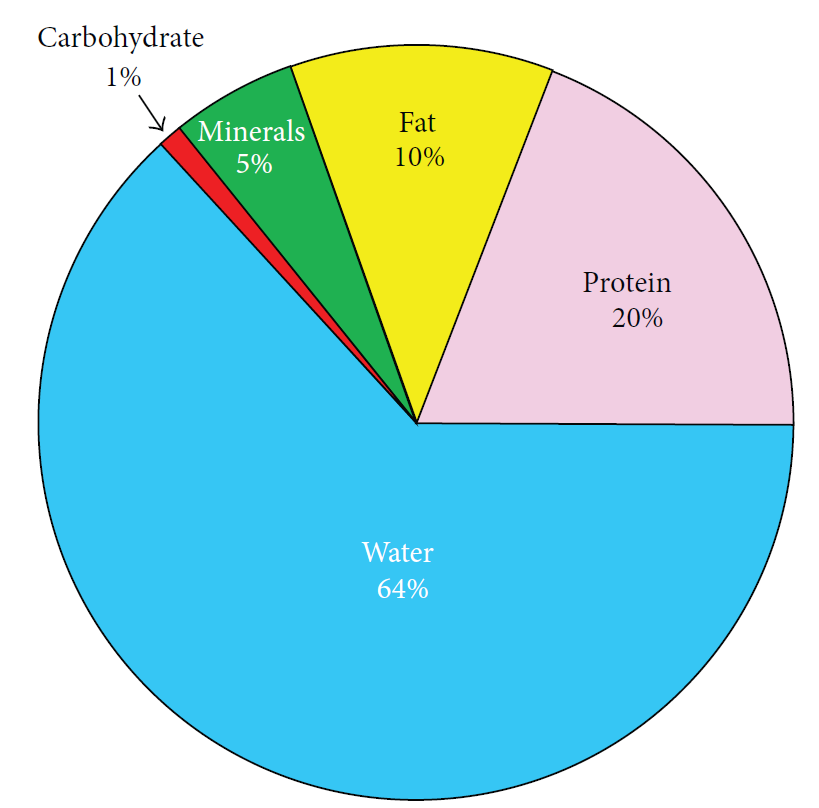
\includegraphics[width=0.5\textwidth]{Figures/sastav_tijela_2.png} 
    \caption{Udio vode, proteina, masti i minerala u ljudskom tijelu \cite{Bera2014}}
    \label{slk:sastav_tijela}
\end{figure}

Sastav ljudskog tijela prikazan je na slici \ref{slk:sastav_tijela}.
Voda je osnovni element stanica i tkiva te je nužna za brojne fiziološke procese u organizmu, 
kao na primjer održavanje elektrolitske ravnoteže i regulacija temperature.
Ukupnu vodu u tijelu (engl. \textit{Total Body Water; TBW}) 
dijelimo na intracelularnu vodu (engl. \textit{Intracellular Water; ICW}) i ekstracelularnu vodu (engl. \textit{Extracellular Water; ECW}) \cite{Bera2014}. 
Važni parametri pri analizi ljudskog tijela su i masa tijela bez masnog tkiva (engl. \textit{Fat Free Mass; FFM}) 
te masa masnog tkiva (engl. \textit{Fat Mass; FM}) \cite{Bera2014}.

Ekstracelularna voda je količina vode koja se nalazi izvan stanica te čini 30-40\% ukupne vode. Uključuje krv, limfu, tekućinu u 
zglobovima i međustaničnom prostoru. Ima važnu ulogu u transportu kisika i hranjivih tvari do stanica te odvođenju otpadnih 
tvari iz organizma \cite{Bera2014}.

Intracelularna voda je voda koja se nalazi unutar citoplazme stanica, predstavljajući ključnu 
komponentu u održavanju stanične homeostaze i omogućavajući različite biokemijske reakcije 
koje su neophodne za životne procese.
Održavanje ravnoteže između ekstracelularne i intracelularne vode ključno je za normalno funkcioniranje organizma \cite{Bera2014}.

Masno tkivo je također važno za funkcioniranje organizma jer pruža energetsku rezervu, toplinsku izolaciju te štiti unutarnje organe. 
Prekomjerno nakupljanje masnoće može dovesti do različitih zdravstvenih problema, poput pretilosti, dijabetesa i 
bolesti kardiovaskularnog sustava. 
Zbog toga je praćenje udjela masnog tkiva u organizmu važno u procijeni rizika od brojnih bolesti \cite{Bera2014}.

Masu tijela bez masnog tkiva dobijemo tako da od ukupne mase tijela oduzmemo masu masnog tkiva. 
FFW uključuje tjelesnu vodu, mišiće, kosti, organe i druga tkiva osim masnih tkiva te predstavlja masu koja je aktivna i sudjeluje 
u metaboličkim procesima \cite{Bera2014}.

\begin{figure}[htb]
    \centering
    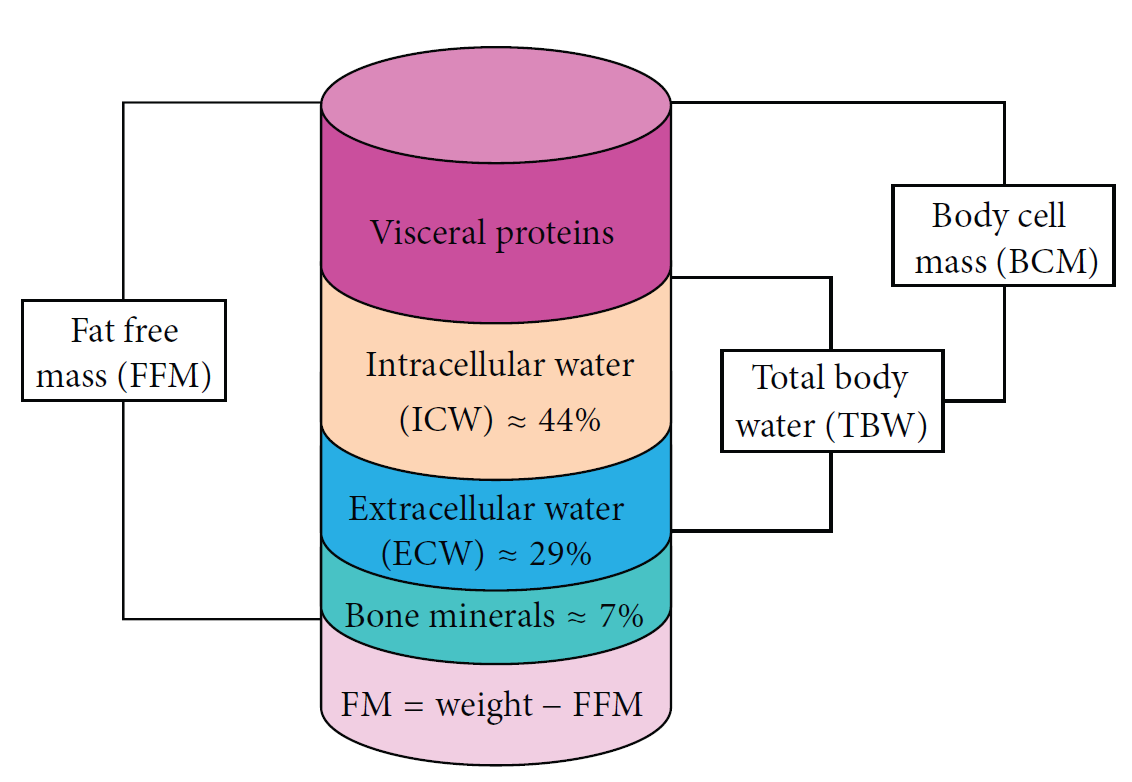
\includegraphics[width=0.85\textwidth]{Figures/sastav_tijela.png} 
    \caption{Sastav ljudskog tijela \cite{Bera2014}}
    \label{slk:sastav_tijela}
\end{figure}

%Koliko dobro će tkivo provoditi struju, ovisi o količini vode u njemu. 
%Tkiva koja imaju više vode u sebi, kao na primjer mišići, bolje provode električnu struju nego masno tkivo koje ne sadrži vodu. 
%Zbog toga se sastav ljudskog tijela procjenjuje iz izmjerene bioimpedancije između različitih dijelova tijela. 
%Iz bioimpedancije sastav tijela se dobiva putem teorijskih jednadžbi ili tablica koje ovise o parametrima 
%kao što su spol, dobna skupina, težina i visina.

\section{Praćenje distribucije tekućine u nogama}

U ovom radu, naglasak je stavljen na praćenje distribucije tekućine u potkoljenici. 
Sastav potkoljenice može se dobiti mjerenjem njezine bioimpedancije te zatim korištenjem teorijskih jednadžbi. 
Prvi korak je određivanja volumena potkoljenice. 
Potkoljenica je aproksimirana cilindrom te se njezin volumen određuje s pomoću jednadžbe \ref{jed:volmen_noge}, 
pri čemu je \textit{L} razmak između naponskih elektroda, a \textit{O} opseg potkoljenice.

\begin{equation}
    \label{jed:volmen_noge}
    \mathrm{V}=L A=L \frac{O^2}{4 \pi}
\end{equation} 

Sljedeći korak je mjerenje bioimpedancije te zatim izračunavanje $R_{0}$ i $R_{\infty}$.
$R_{0}$ i $R_{\infty}$ predstavljaju otpor tkiva na nultoj i beskonačnoj frekvenciji te će detaljno biti opisani u poglavlju \ref{chap:bioz}.

Za izračunavanje volumena TBW, ECW i ICW u potkoljenici korištene su formule opisane u \cite{Delano2022}:
\begin{equation}
    \label{jed:ecw_noge}
    ECW=\frac{1}{1000} *\left(\frac{\rho_e L^2 \sqrt{V}}{R_0}\right)^{\frac{2}{3}}
\end{equation} 
\begin{equation}
    \label{jed:tbw_noge}
    TBW=\frac{1}{1000} *\left(\frac{\rho_{\infty} L^2 \sqrt{V}}{R_{\infty}}\right)^{\frac{2}{3}}
\end{equation} 
\begin{equation}
    \label{jed:icw_noge}
    ICW=TBW-ECW 
\end{equation} 
pri čemu je $\rho_{e}$ efektivna otpornost ekstracelularne tekućine iznosa 273,9 $\Omega$cm, a 
$\rho_{\infty}$ efektivna otpornost ukupne tjelesne tekućine iznosa 937,2 $\Omega$cm.
Sve jedinice izražene su u centimetrima te ukupni volumen dobivamo u centimetrima kubičnim. 
Kako bi konačan rezultat bio u litrama dijelimo ga s 1000. 

\end{document}